\documentclass[12pt, a4paper]{article}

% --- Pacotes Essenciais ---
\usepackage[brazil]{babel}
\usepackage[utf8]{inputenc}
\usepackage[T1]{fontenc}
\usepackage{amsmath}
\usepackage{amssymb}
\usepackage{enumitem} % Pacote para personalizar listas
\usepackage{graphicx}
\usepackage{tabularx}
\usepackage{subcaption} % no preâmbulo
\usepackage{booktabs}
\usepackage[a4paper,
    left=3cm,
    right=2cm,
    top=3cm,
    bottom=2cm]{geometry}
\usepackage{hyperref}
\usepackage{booktabs}
\usepackage{fancyhdr}
\usepackage[alf]{abntex2cite} % Citações padrão ABNT (Autor-Data)
\usepackage{booktabs}
\usepackage{siunitx} % Para alinhar números pelas casas decimais, se desejar
\setlength{\parindent}{0pt}  % Comando para remover o recuo da primeira linha
% --- Configuração do Cabeçalho (Modificada) ---
\pagestyle{fancy}
\fancyhf{} % Limpa tudo, exceto o rodapé que vamos definir abaixo
\setlength{\headheight}{18pt} 
\renewcommand{\headrulewidth}{0.4pt} 

% --- DEFINIÇÃO DO CABEÇALHO ---
\fancyhead[L]{
    
\includegraphics[height=1.0cm]{image/LOGOBAS.png}
    }

\fancyhead[R]{
    \textbf{BAS ENGENHARIA LTDA}\\
    \small CEL: (11) 96594-2163 // \href{mailto:BRUNO@BASENGENHARIA.COM}{BRUNO@ENGENHARIA.COM}
    }
% --- INSERIR NÚMERO DA PÁGINA NO RODAPÉ ---
\fancyfoot[C]{\thepage} % Centraliza o número da página no rodapé
% --- ESTILO PARA PÁGINAS INICIAIS (TOC e Chapters) ---
\fancypagestyle{plain}{
    \fancyhead{} % Limpa completamente o cabeçalho
    \fancyfoot{}
    \renewcommand{\headrulewidth}{0pt} % Remove a linha separadora
}

% Renomear "Conteúdo" para "Sumário"
\addto\captionsbrazil{\renewcommand{\contentsname}{Sumário}}

% --- CORREÇÃO DE CONFLITO DE ALTURA ---
\geometry{
    a4paper,
    top=3cm,
    bottom=3cm,
    left=3cm,
    right=2cm,
    headheight=18pt, % Alterado para 18pt para resolver o conflito com \headheight
}

% --- Início do Documento ---
\begin{document}
\begin{titlepage}
    \centering

    % Título no topo
    \vspace{1cm}
    \begin{center}
        {\Large{LAUDO TÉCNICO}}\\
        {\Large{ANÁLISE ESTRUTURAL DE PÓRTICO}\\
        {\Large{METÁLICO POR ELEMENTOS FINITOS}}
    \end{center}
    
    \vfill % Empurra o restante para baixo
    \begin{figure}[h!]
        \centering
        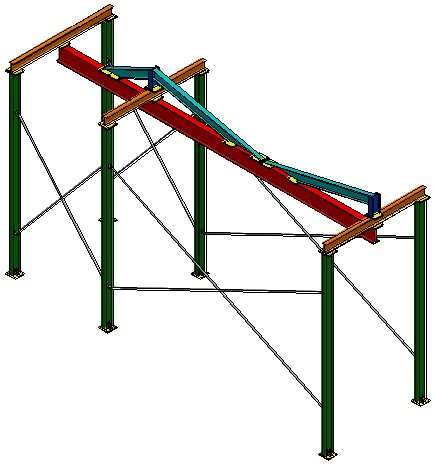
\includegraphics[width=0.75\linewidth]{image/portico.jpg}
        %\caption{Caption}
        \label{fig:placeholder}
    \end{figure}
    
    % Informações Técnicas
    \begin{center}
        {\Large \textbf{N\textsuperscript{o} DO LAUDO:} LT30032026}\\[1mm]
        {\Large \textbf{ENGENHEIRO RESPONSÁVEL:} Bruno Almeida Silva}\\[1mm]
        {\Large \textbf{CREA/SP:} 5069978388}\\
    \end{center}
    
    \vfill % Empurra a data para o final
    
    % Data no fim da página (Adicionado)
    {\large \today} 

\end{titlepage}
\clearpage
% Sumário
\tableofcontents
\newpage

% ------------------------------------------------------
% 1. IDENTIFICAÇÃO DO PROJETO
% ------------------------------------------------------
\section{IDENTIFICAÇÃO DO PROJETO}

\begin{itemize}
    \item \textbf{Projeto:} Pórtico Metálico Regular
    \item \textbf{Capacidade de Carga:} 10t
    \item \textbf{Data do Laudo:} 30/03/2026
\end{itemize}

\subsection{Dados da Empresa}

\begin{itemize}
    \item \textbf{Razão Social:} CONSORCIO TELAR VELLOSO VAD PACOTE 21
     \item \textbf{CNPJ:} 58.525.894/001-13
     \item \textbf{Endereço:} AV. ANGÉLICA, 2510, 2º andar, Consolação, São Paulo - SP
     \item \textbf{CEP:} 01228-200\\
\end{itemize}

\subsection{Dados do Prestador}
\begin{itemize}
    \item \textbf{Razão Social:} BAS ENGENHARIA LTDA
    \item \textbf{CNPJ:} 35.726.144/001-4
    \item \textbf{Endereço:} R. ANTONIO ALFREDO CAMPOS S/N - JARDIM GUANHEMBU
    \item \textbf{CEP:} 04814 - 560
    \item \textbf{Email:} bruno@basengenharia.com\\
\end{itemize}
%\textbf{Obra/Local:}

\newpage

% ------------------------------------------------------
% Objetivo
% ------------------------------------------------------

\section{OBJETIVO}

O presente relatório tem por finalidade avaliar a segurança estrutural de um pórtico metálico destinado à fabricação, submetido às condições de carregamento de projeto.

A análise estrutural foi realizada por meio de modelagem numérica utilizando o Método dos Elementos Finitos, considerando comportamento elástico linear do material e hipóteses de pequenos deslocamentos.

Foram determinados deslocamentos, esforços internos e tensões atuantes, com posterior verificação quanto aos critérios de resistência estabelecidos pelas normas técnicas aplicáveis.

Adicionalmente, foi conduzida análise de flambagem linear com o objetivo de determinar os fatores críticos de carga e avaliar a estabilidade global da estrutura.

Os resultados obtidos subsidiam a validação do dimensionamento estrutural e a liberação do projeto para fabricação.
\section{Geometria da Estrutura}

A geometria analisada corresponde a um pórtico metálico tridimensional, modelado como sólido 3D, representando colunas, vigas e travamentos estruturais. A configuração geométrica foi desenvolvida no ANSYS, conforme ilustrado na Figura ~\ref{fig:portico3D}, com dimensões definidas para reproduzir as condições reais de projeto.

O modelo foi concebido para representar adequadamente o comportamento estrutural global, a rigidez do sistema e a distribuição dos esforços internos, adotando-se simplificações compatíveis com a hipótese de comportamento linear elástico e pequenos deslocamentos.

As ligações estruturais foram consideradas conectadas, e as bases modeladas como engastadas, conforme hipóteses descritas na seção de condições de contorno.

\begin{figure}[h!]
    \centering
    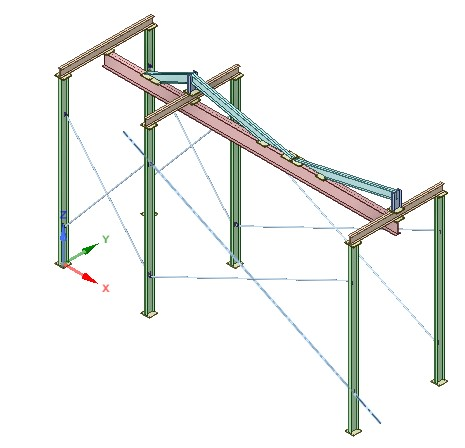
\includegraphics[width=0.75\linewidth]{image/portico3D.jpg}
    \caption{Pórtico sólido 3D.}
    \label{fig:portico3D}
\end{figure}
% ============================================================
% SEÇÃO: Materiais
% ============================================================

\section{Material Utilizado na Análise}

Os materiais empregados na análise foram definidos no módulo de dados do ANSYS, com base nas propriedades elásticas isotrópicas do aço estrutural selecionado. Os parâmetros mecânicos relevantes incluem módulo de elasticidade, módulo de cisalhamento, coeficiente de Poisson e densidade, conforme apresentado nas Tabelas ~\ref{tab:astm_a36_analysis} e ~\ref{tab:astm_a572_gr50}.

%==================================================================
%Tabela das propriedades do aço A36
\begin{table}[ht]
\centering
\caption{Propriedades mecânicas e físicas do aço ASTM A36 adotadas na análise}
\label{tab:astm_a36_analysis}
\renewcommand{\arraystretch}{1.2}

\begin{tabularx}{0.75\textwidth}{|l|c|X|}
\toprule
\textbf{Propriedade} & \textbf{Unidade} & \textbf{Valor} \\
\midrule
Densidade & kg/m$^3$ & 7\,850 \\
Módulo de Young ($E$) & GPa & 200 \\
Coeficiente de Poisson ($\nu$) & -- & 0,26 \\
Módulo de cisalhamento ($G$) & GPa & 79,3 \\
Resistência ao escoamento ($f_y$) & MPa & 250 (mín.) \\
Resistência última à tração ($f_u$) & MPa & 400--550 \\
\bottomrule
\end{tabularx}
\end{table}
%========================================================================
%Tabela de propriedades aço A572
\begin{table}[ht]
\centering
\caption{Propriedades físicas e mecânicas do aço ASTM A572 Grade 50 adotadas na análise}
\label{tab:astm_a572_gr50}
\renewcommand{\arraystretch}{1.2}

\begin{tabularx}{0.75\textwidth}{|l|c|X|}
\toprule
\textbf{Propriedade} & \textbf{Unidade} & \textbf{Valor} \\
\midrule
Densidade & kg/m$^3$ & 7\,850 \\
Módulo de Young ($E$) & GPa & 200 \\
Coeficiente de Poisson ($\nu$) & -- & 0,3 \\
Módulo de cisalhamento ($G$) & GPa & 79,3 \\
Resistência ao escoamento ($f_y$) & MPa & 345 (mín.) \\
Resistência última à tração ($f_u$) & MPa & 450--620 \\
\bottomrule
\end{tabularx}
\end{table}


% ============================================================
% SEÇÃO: Conexões
% ========================================================================================================================
% SEÇÃO: Malha
% ============================================================

\newpage
\section{Discretização e Qualidade da Malha}

A discretização do domínio computacional foi realizada por meio de elementos sólidos, disponíveis na formulação padrão do \textbf{ANSYS Mechanical}. Estes elementos possuem seis graus de liberdade por nó ($u_x, u_y, u_z, \theta_x, \theta_y, \theta_z$), permitindo a captura adequada de gradientes de tensão e fenômenos de instabilidade local, conforme detalhado na Tabela~\ref{tab:config_malha}.

A malha foi gerada de forma estruturada nas mesas e almas dos perfis, utilizando um comprimento de elemento uniforme de $250,0$~mm. Tal refinamento foi definido com base em um estudo de convergência prévio, visando assegurar a independência dos resultados em relação ao tamanho da discretização e garantir a precisão na transição de esforços entre os componentes do pórtico.

\begin{table}[ht]
\centering
\caption{Parâmetros da discretização adotada}
\label{tab:config_malha}
\renewcommand{\arraystretch}{1.2}

\begin{tabularx}{0.7\textwidth}{|l|X|}
\toprule
\textbf{Parâmetro} & \textbf{Valor} \\
\midrule
Tipo de elemento & Sólido \\
Comprimento médio do elemento & $\sim250 mm \\
Critério de refinamento & Tamanho uniforme \\
Número total de elementos & 22288 \\
Número total de nós & 113491 \\
\bottomrule
\end{tabularx}
\end{table}
% ------------------------------------------------------
% 4. NORMAS APLICADAS
% ------------------------------------------------------
 
% SEÇÃO: Análise Estática Estrutural
% ============================================================

\section{Condições de Contorno e Vínculos Estruturais}

As condições de contorno aplicadas às bases do pórtico adotaram a hipótese de \textbf{engastamento perfeito} (\textit{Fixed Support}). Esta configuração impõe restrições cinemáticas totais aos seis graus de liberdade (6 DOF) nos nós de apoio, conforme detalhado abaixo:

\begin{itemize}
    \item \textbf{Translações:} Restrição completa nos eixos $u_x, u_y$ e $u_z$ (anulação de deslocamentos lineares);
    \item \textbf{Rotações:} Restrição completa em torno dos eixos $\theta_x, \theta_y$ e $\theta_z$ (impedimento de giros).
\end{itemize}

Tal premissa de modelagem assume que o conjunto formado pela placa de base, chumbadores de ancoragem e bloco de fundação possui rigidez suficiente para absorver os momentos fletores resultantes, garantindo a estabilidade global da estrutura e a fidelidade aos esforços calculados na interface com o solo.

\subsection{Definição dos Carregamentos e Condições de Solicitação}

O carregamento externo foi estabelecido para simular a ação operacional máxima de içamento. A solicitação foi modelada como uma força concentrada de \textbf{178,542 kN} (correspondente a 10 tf majoradas pelos fatores de majoração e dinâmico(ver Tabela ~\ref{carreg}, aplicada verticalmente no sentido negativo do eixo-z ($F_z$).

Para garantir a transmissão realista dos esforços e evitar singularidades numéricas (picos de tensão artificiais), utilizou-se o recurso de acoplamento cinemático (\textit{Remote Force} ou \textit{RBE3}), distribuindo a carga na região de contato do elemento de suspensão. Esta metodologia assegura que o vetor de carga seja transferido integralmente à seção transversal da viga principal, respeitando a excentricidade prevista em projeto.

\begin{table}[h!]
\centering
\caption{Carregamentos estruturais aplicados}
\label{carreg}
\renewcommand{\arraystretch}{1.2}

\begin{tabularx}{0.85 \textwidth}{|l|c|X|}
\toprule
\textbf{Propriedade} & \textbf{Magnitude} & \textbf{Unidade} \\ 
\midrule
Carga útil considerada & 10 & t \\[4pt]

Conversão para Newtons & 98,1 & kN\\[4pt]

Fator de majoração (ELU-NBR 8800) & 1.4 & \\[4pt]

Fator dinâmico (içamento com movimento) & 1.3 &\\[4pt]

Carga total para simulação & 18,2 & t\\[4pt]

Carga equivalente em Newtons & 178,542 & kN\\[4pt]

Gravidade & 9.81 &  $m/s^{2}$\\

\bottomrule
\end{tabularx}

\end{table}

\begin{figure}
    \centering
    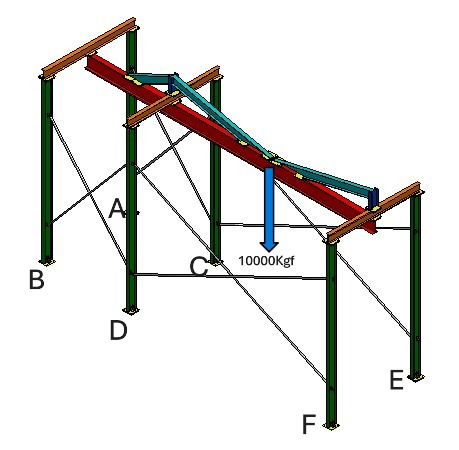
\includegraphics[width=0.75\linewidth]{image/portico-3D.jpg}
    \caption{Carregamentos e localização das bases do pórtico.}
    \label{fig:placeholder}
\end{figure}
\subsection{Metodologia Numérica e Algoritmos de Solução}

A avaliação da integridade estrutural foi realizada via Método dos Elementos Finitos (MEF), utilizando o solver \textit{Sparse Direct} do software ANSYS Mechanical. 

Para a análise estática, adotou-se uma formulação \textbf{linear elástica}, adequada ao regime de pequenas deformações previsto para a estrutura. A solução do sistema de equações lineares foi obtida em etapa única, garantindo a convergência direta dos deslocamentos e esforços internos.

Posteriormente, realizou-se uma análise de \textbf{instabilidade elástica} (\textit{Linear Buckling}) via método de autovalores (\textit{Lanczos}). Este procedimento permitiu a extração dos modos críticos de flambagem e seus respectivos fatores de carga ($\lambda_{cr}$), calculados a partir da matriz de rigidez geométrica gerada pelo estado de tensões da análise estática precedente.

% ============================================================
% SEÇÃO: Resultados da Análise Estática
% ============================================================
\section{Resultados e Verificações Normativas}

Nesta seção, os dados extraídos da simulação numérica são confrontados com os limites estabelecidos pela \textbf{NBR 8800:2008}, visando a validação da estrutura e segurança nos Estados Limites Último (ELU) e de Serviço (ELS).

% ------------------------------------------------------
% SEÇÃO ESPECIAL: DETERMINAR SE O MATERIAL ROMPEU
% ------------------------------------------------------
\subsection{Estado Limite Último - Resistência e Combinação de Ações}

Para a verficação de resistência, a carga norminal de içamento ($P_n=9,81kN$) foi majorada considerando-se os coeficientes de ponderação das ações e o efeito dinâmico do equipamento. A carga de projeto ($F_{sd}$) foi definida por:

\begin{equation}
    F_{sd} = P_n \times \gamma_f \times \gamma_d = 100\text{ kN} \times 1,4 \times 1,3 = 178542\text{ N}
\end{equation}

Onde $\gamma_f = 1,4$ é o coeficiente de ponderação para ações variáveis e $\gamma_d = 1,3$ é o coeficiente de impacto dinâmico. A condição de segurança estabelece que a tensão de Von Mises ($\sigma_{vm}$) não deve ultrapassar a resistência de cálculo do aço.

Critério segundo a NBR 8800, para ELU:

\begin{equation}
    \frac{\sigma_{vm}}{f_{y}/\gamma_{a}} \le 1,0
\end{equation}

onde:

\begin{itemize}
    \item $\sigma_{vm}$: tensão de von Mises
    \item  $f_{y}$: resistência ao escoamento do aço
    \item $\gamma_{a}$: coeficiente parcial do material
\end{itemize}

Para o aço ASTM A572 Gr. 50, $f_y=345MPa$ com $\gamma_a=1,1$.
A Tabela~\ref{tab:verificacao_elu} apresenta os valores máximos de tensão obtidos e os respectivos limites normativos, permitindo verificar a manutenção do comportamento elástico da estrutura.

\begin{table}[ht]
\centering
\caption{Verificação do comportamento elástico — Estado Limite Último (ELU)}
\label{tab:verificacao_elu}
\renewcommand{\arraystretch}{1.2}

\begin{tabularx}{0.6 \textwidth}{|l|X|}
\toprule
\textbf{Grandeza} & \textbf{Valor}\\
\midrule
Tensão de von Mises Máxima& 146,6 MPa \\

Resistência de cálculo 
$\displaystyle \frac{f_y}{\gamma_a}$ & 313,6 MPa \\

Situação & \textbf{Atende} \\
\bottomrule
\end{tabularx}
\end{table}

\begin{figure}[h!]
    \centering
    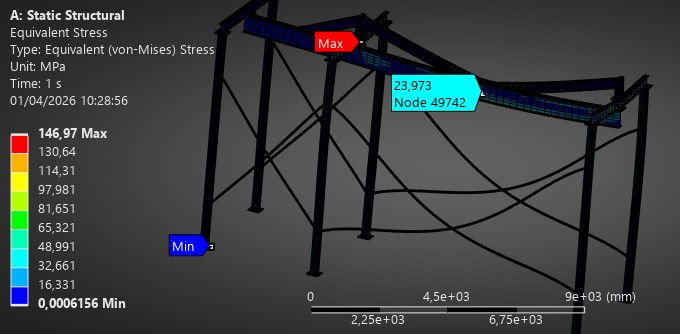
\includegraphics[width=0.85\linewidth]{image/von-mises.jpg}
    \caption{Tensão de von Mises.}
    \label{fig:placeholder}
\end{figure}

\subsection{Estado Limite de Serviço - Verificação de Flechas}

A verificação de serviço visa garantir a funcionalidade operacional. Para esta análise, utilizam-se as cargas nominais (sem majoração de $\gamma_f$), conforme preconiza a norma para verificações de utilização.

Critério:

\begin{equation}
    \delta_{max} \le \delta_{adm} = \frac{L}{300}
\end{equation}

A tabela~\ref{tab:verificacao_els} apresenta os valores obtidos e os respectivos limites adotados, permitindo a verificação da conformidade da estrutura quanto aos critérios de serviço.

\begin{table}[h!]
\centering
\caption{Verificação dos deslocamentos — Estado Limite de Serviço (ELS)}
\label{tab:verificacao_els}
\renewcommand{\arraystretch}{1.2}

\begin{tabularx}{0.85\textwidth}{|l|c|c|X|}
\toprule
\textbf{Grandeza} &
\textbf{Valor máximo} &
\textbf{Valor admissível} &
\textbf{Situação} \\
\midrule
Flecha Máxima & 
$\;\;\;$ 10,4mm & 
$L/300\;\;\;$ = $\;\;\;$ 31,7mm & 
\textbf{Atende} \\
\bottomrule
\end{tabularx}
\end{table}

\begin{figure}[h!]
    \centering
    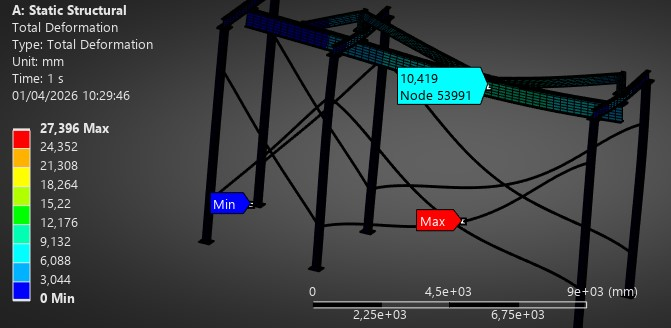
\includegraphics[width=0.85\linewidth]{image/total-deformation.jpg}
    \caption{Caption}
    \label{fig:placeholder}
\end{figure}

\subsection{Estabilidade Elástica - Fator de Carga Crítica}

A estabilidade global é avaliada pelo autovalor $\lambda_{cr}$ decorrente da análise de flambagem estrutural sob os carregamentos considerados. Este valor indicar a reserva de segurança contra flambagem para a combinação de carga total aplicada.

Critério típico:

\begin{equation}
    \lambda_{cr}>1,0
\end{equation}

O resultado da análise de flambagem mostrou, conforme Tabela \ref{tab:buckling_modes}, que:

\begin{table}[h!]
    \centering
    \caption{Fatores de Carga Crítica (Autovalores) - Análise de Flambagem Linear}
    \label{tab:buckling_modes}
    \begin{tabular}{@{}ccc@{}}
        \toprule
        \textbf{Modo} & \textbf{Fator de Carga ($\lambda$)} & \textbf{Status de Instabilidade} \\ \midrule
        1 & -10,007 & Flambagem Inversa (Irrelevante) \\
        2 & -5,5933 & Flambagem Inversa (Irrelevante) \\
        3 & -3,7586 & Flambagem Inversa (Irrelevante) \\ \midrule
        \textbf{4} & \textbf{6,4912} & \textbf{1º Modo Crítico (Global)} \\
        5 & 6,7077 & 2º Modo Crítico \\
        6 & 8,9516 & 3º Modo Crítico \\
        7 & 10,398 & 4º Modo Crítico \\
        8 & 11,486 & 5º Modo Crítico \\
        9 & 11,543 & 6º Modo Crítico \\
        10 & 12,254 & 7º Modo Crítico \\ \bottomrule
    \end{tabular}
    \vspace{0.2cm}
    \small \\ \textit{Nota: O fator crítico global de \textbf{6,49} indica que a estrutura suporta teoricamente 6,49 vezes a carga nominal antes da instabilidade elástica.}
\end{table}
\newpage

Com base nos resultados apresentados, verifica-se que as tensões normais combinadas permaneceram inferiores ao limite de escoamento do material, os deslocamentos máximos atenderam aos critérios estabelecidos para os estados limites de serviço e os fatores de carga críticos obtidos na análise de flambagem foram superiores à unidade. Dessa forma, conclui-se que a estrutura apresentou comportamento predominantemente elástico, não sendo identificados indícios de plastificação, deformações permanentes ou instabilidade elástica nas condições analisadas.

\begin{figure}[h!]
    \centering
    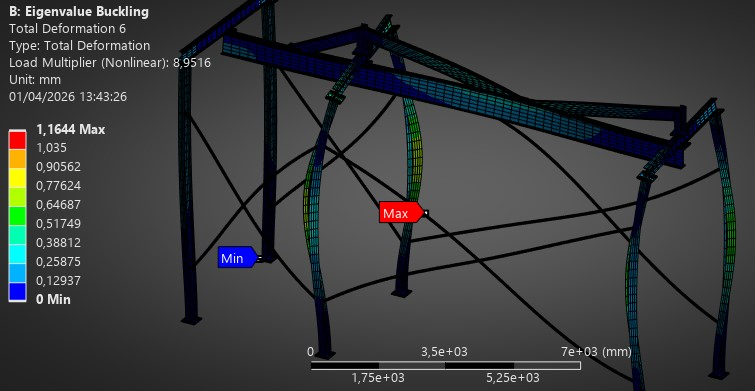
\includegraphics[width=0.75\linewidth]{image/modo-critico.jpg}
    \caption{1º Modo Crítico global de flambagem.}
    \label{fig:placeholder}
\end{figure}

% ============================================================

% ============================================================

% 7. FORÇAS DE REAÇÃO NOS APOIOS
% ------------------------------------------------------
\section{Reações de Apoio e Verificações das Conexões}

A análise das reações de apoio é fundamental para o dimensionamento dos elementos de fixação (parafusos/chumbadores) e validação do equilíbrio estático global da estrutura sob carga majorada ($F_{sd}=178542N$).

As reações foram extraídas nas superfícies (Shell) das bases onde aplicou-se a condição de \textit{Fixed Support}. Os valores representam a somatória dos esforços por pilar, garantindo o equilíbrio:

\begin{equation}
\sum \vec{F} = \vec{0}
\quad \text{e} \quad
\sum \vec{M} = \vec{0}
\end{equation}



% ------------------------------------------------------
% Reações
% ------------------------------------------------------

\begin{figure}[h!]
    \centering
    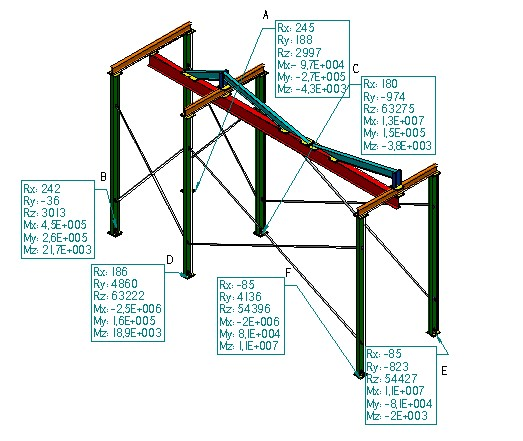
\includegraphics[width=0.75\linewidth]{image/reacoes.jpg} % Ajustado para 1.0
    \caption{Resultados das reações por base. $[R_{i}]=N$; $[M_{i}]=N \cdot mm$}
    \label{fig:reacoes}
\end{figure}

\begin{table}[h!]
    \centering
    \caption{Reações de Apoio nas Bases do Pórtico (6 Pontos de Contato)}
    \label{tab:reacoes_6_bases}
    \renewcommand{\arraystretch}{1.2}
    
    \begin{tabular}{|l|c|c|}
        \toprule
        \textbf{Identificação} & \textbf{Reação Normal ($F_z$)} & \textbf{Esforço Cortante ($V_{xy}$)} \\ 
        \textbf{da Base} & [N] & [N]\\ \midrule
        Base A   & 2997 & 309\\
        Base B   & 3013 & 302\\
        Base C   & 63275 & 4873\\
        Base D   & 63222 & 4863\\
        Base E   & 54427 & 4155 \\
        Base F   & 54396 & 4158 \\ 
        \bottomrule
        
    \end{tabular}
    \vspace{0.2cm}
\end{table}



\begin{table}[h!]
\centering
\caption{Propriedades do parafuso M24 classe 10.9}
\label{tab:propriedades_parafuso}
\renewcommand{\arraystretch}{1.2}

\begin{tabular}{|l|c|c|}
\toprule
\textbf{Parâmetro} & \textbf{Valor} & \textbf{Unidade} \\
\midrule
Diâmetro nominal ($d$) & 24 & mm \\
Área resistente ($A_s$) & 353 & mm$^2$ \\
Limite de escoamento ($\sigma_{y}$) & 940 & MPa \\
Resistência última à tração ($\sigma_{u}$) & 1040 & MPa \\
Coeficiente parcial de segurança ($\gamma$) & 1,4 & -- \\
Quantidade de parafusos & 4 & unidades \\
\bottomrule
\end{tabular}
\end{table}

\subsection{Cálculo da Carga Admissível por Parafuso}

A capacidade resistente dos parafusos foi avaliada separadamente para esforços de tração e cisalhamento, adotando-se os critérios de resistência elástica com aplicação do coeficiente parcial de segurança do material.

\subsubsection{Verificação à Tração}

A força resistente de cálculo à tração por parafuso ($F_{f,Rd}$) foi determinada conforme as prescrições da NBR 8800, considerando o limite de ruptura do aço classe 10.9 e fator de redução de eficiência:

\begin{equation}
F_{t,Rd} = \frac{0,75 \cdot \sigma_{y} \cdot A_s}{\gamma_{a2}}
\end{equation}

Substituindo-se os valores adotados:

\begin{equation}
F_{t,Rd} = \frac{0,75 \times 940 \times 353}{1{,}4}  \approx 177{,}8 \, \text{KN}
\end{equation}

\subsubsection{Verificação ao Cisalhamento}

Para o cisalhamento, considera-se a resistência equivalente a 60\% do limite de escoamento, conforme prática consagrada em normas de projeto:

\begin{equation}
F_{v,Rd} = \frac{0.4 \cdot \sigma_{y} \cdot A_s}{\gamma}
\end{equation}

Resultando em:

\begin{equation}
V_{v,Rd} = \frac{0{,}4 \times 940 \times 353}{1{,}4} \approx 94{,}8 \, \text{KN}
\end{equation}

% ------------------------------------------------------
% 9. VALIDAÇÃO DOS PARAFUSOS DA MONOVIA
% ------------------------------------------------------
O critério de segurança baseia-se na equação de interação para solicitações combinadas, onde a soma das razões de utilização deve ser inferior ou igual a 1,0 por parafuso:

\begin{equation}
    \eta = \left( \frac{F_{t,Sd}}{F_{t,Rd}} \right) + \left( \frac{F_{v,Sd}}{F_{v,Rd}} \right) \leq 1,0
\end{equation}

\vspace{0.5cm}

\begin{table}[h]
\centering
\caption{Resultados do critério de segurança de carga admissível por parafuso em cada base.}
\label{tab:verificacao_bases}
\begin{tabularx}{0,78\textwidth}{|l|c|c|C|C|}
\toprule
\textbf{Localização} & {\textbf{$F_{t,Sd}$ [N]}} & {\textbf{$F_{v,Sd}$ [N]}} & {\textbf{Verificação ($\eta$)}} & \textbf{Status} \\ \midrule
Base A & 749 & 77 & 5E-3 & \textbf{Aprovado}\\
Base B & 753 & 75 & 5E-03 & \textbf{Aprovado} \\
Base C & 15819 & 1218 & 1E-1 & \textbf{Aprovado}\\
Base D & 15806 & 1216 & 1E-1 & \textbf{Aprovado}\\
Base E & 13607 & 1039 & 9E-02 & \textbf{Aprovado}\\
Base F & 13599 & 1039 & 9E-02 & \textbf{Aprovado}\\
\bottomrule
\end{tabularx}
\end{table}

\section*{Análise dos Resultados}
Conforme apresentado na Tabela \ref{tab:verificacao_bases}, o coeficiente de utilização máximo ($\eta_{max}$) foi identificado nas \textbf{Bases 3 e 4}, atingindo aproximadamente \textbf{9,8\%} da capacidade nominal do conjunto de fixação. A folga de segurança de 90,2\% garante a integridade da estrutura mesmo sob eventuais efeitos dinâmicos de içamento.

Conclui-se, portanto, que a ligação analisada atende aos critérios de segurança estrutural estabelecidos pelas normas técnicas aplicáveis, sendo considerada segura para as condições de carregamento avaliadas na simulação numérica.


\newpage
% ------------------------------------------------------
% 10. RECOMENDAÇÕES DE SOLDAGEM
% -----------------------------------------------------

% ------------------------------------------------------
% 12. CONCLUSÃO
% ------------------------------------------------------
\section{Conclusão}

A análise estrutural conduzida permitiu avaliar o comportamento do pórtico metálico sob
carregamento estático e investigar sua suscetibilidade à instabilidade por flambagem. Os
resultados obtidos demonstraram que:

\begin{itemize}
    \item As tensões equivalentes críticas permaneceram significativamente abaixo do
    limite de escoamento do aço, indicando que a estrutura opera integralmente     no regime elástico.
    
    \item O deslocamento máximos obtidos, 11,4mm, foi inferiore ao limite admissível estabelecido pelo critério $L/300$, garantindo desempenho adequado e segurança operacional durante o içamento e locomoção de cargas.
    
    \item A análise de flambagem linear evidenciou modo crítico com cargas de instabilidade superiores à carga de serviço considerada,  com margem de segurança contra instabilidades globais.
    
    \item A verificação dos elementos de fixação, incluindo parafusos M24 classe 10.9, confirmou capacidade resistente adequada frente às solicitações de tração e cisalhamento,
    atendendo às prescrições normativas.
\end{itemize}

A partir dos resultados, conclui-se que o pórtico metálico LT30032026 apresenta comportamento estrutural seguro e compatível com os critérios de resistência e estabilidade adotados. A estrutura encontra-se validada para a capacidade de carga
especificada (10t), não havendo indícios de plastificação ou instabilidade que comprometam sua integridade.

% ------------------------------------------------------
% 13. AUTORIZAÇÃO PARA MODIFICAÇÕES FUTURAS


% ------------------------------------------------------
% 14. APENDICE
% ------------------------------------------------------


% ------------------------------------------------------
% 14. 
% ------------------------------------------------------
\section{Recomendações}
Itens verificados na inspeção 
\begin{itemize}
    \item Alinhamento e nivelamento da estrutura
    \item Presença de fissuras, empenamentos ou deformações
    \item Condidções das soldas (inspeção visual e LP em pontos críticos)
    \item Aperto e integridade dos parafusos M24 (torque e tração)
    \item Estado da pintura anticorrosiva e presença de pontos de oxidação
    \item Fixação da chapa base e integridade dos chumbadores
\end{itemize}

\begin{enumerate}[label=\alph*)]
    \item Frequência das Inspeções
    \begin{itemize}
        \item Inspeção Visual: Mensal
        \item Inspeção Visual: Semestral
    \end{itemize}

    \item Itens a Serem Verificados na inspeção
    \begin{itemize}
        \item Alinhamento e nivelamento da estrutura
        \item Presença de fissuras, empenamentos ou deformações
        \item Condições de soldas (inspeções visuais)
        \item Estado da pintura anticorrosiva e presença de pontos de oxidação
        Fixação da chapa base e integridade ddos chumbadores
        \item Verificação do aperto dos parafusos e orcas da estrutura (semestral)
    \end{itemize}
\end{enumerate}

\section{Normas Técnicas Adotadas}

O presente relatório foi desenvolvido com base em normas técnicas brasileiras vigentes, com o objetivo de assegurar a consistência metodológica, a confiabilidade das análises numéricas e a adequada avaliação da segurança estrutural dos modelos estudados. As normas adotadas fornecem diretrizes tanto para a modelagem computacional por meio do Método dos Elementos Finitos quanto para a verificação estrutural de elementos em aço.

A adoção conjunta das normas ABNT NBR 16239:2013 e ABNT NBR 8800:2008 garante que o modelo numérico e os procedimentos de verificação empregados estejam alinhados às boas práticas da engenharia estrutural, conforme estabelecido pela :contentReference[oaicite:0]{index=0}.

\subsection{ABNT NBR 16239:2013 — Modelagem por Elementos Finitos}

A ABNT NBR 16239:2013 \cite{nbr16239} estabelece recomendações para a utilização do Método dos Elementos Finitos (MEF) na análise estrutural, abrangendo aspectos relacionados à discretização do modelo, seleção do tipo de elemento, definição das propriedades dos materiais, aplicação das condições de contorno e interpretação dos resultados numéricos.

No presente trabalho, essa norma foi adotada como referência para a definição da estratégia de modelagem estrutural, incluindo a utilização de elementos do tipo viga (\textit{beam elements}) para a representação do pórtico metálico, bem como para a correta aplicação de cargas e vínculos. A interpretação dos resultados foi realizada de forma crítica, considerando as hipóteses e limitações inerentes à análise numérica linear.

\subsection{ABNT NBR 8800:2008 — Projeto de Estruturas de Aço}

A ABNT NBR 8800:2008 \cite{nbr8800} estabelece os critérios e procedimentos para o projeto e a verificação da segurança de estruturas de aço e estruturas mistas de aço e concreto, fundamentados nos conceitos de estados limites últimos (ELU) e estados limites de serviço (ELS).

No presente relatório, essa norma foi empregada como base para a avaliação da segurança estrutural dos elementos analisados, considerando as tensões normais resultantes da combinação de esforços axiais e fletores. Em função da modelagem por elementos de viga, a verificação da resistência foi realizada com base nas tensões normais combinadas nas fibras extremas das seções transversais, procedimento compatível com a filosofia da norma para elementos lineares.

Adicionalmente, os deslocamentos e deformações obtidos nas análises foram avaliados à luz dos critérios de serviço estabelecidos pela NBR 8800, assegurando que o comportamento da estrutura permaneça adequado sob os carregamentos considerados.

\subsection{Referência técnica complementar}

Além das normas brasileiras adotadas, o desenvolvimento das análises relacionadas à transferência de esforços para a fundação, incluindo o comportamento de placas de base e chumbadores, foi fundamentado em literatura técnica consagrada, com destaque para a obra \textit{Base Plate and Anchor Rod Design} \cite{aisc_dg1}.

Essa referência foi utilizada como suporte teórico complementar para a compreensão dos mecanismos de distribuição de tensões de contato, esforços nos chumbadores e verificação da estabilidade local das ligações, contribuindo para a interpretação dos resultados numéricos e para a validação conceitual das soluções adotadas. Ressalta-se que sua utilização teve caráter complementar, não substituindo os critérios normativos estabelecidos pelas normas brasileiras vigentes.

\postextual
\bibliographystyle{abntex2-alf} % Certifique-se de ter o estilo abntex2
\bibliography{referencias} % O nome do seu arquivo .bib
\newpage
\thispagestyle{empty} % remove numeração de página

\vspace*{5cm} % espaço do topo

\begin{tabular}{@{} m{8cm}<{\centering} m{7cm}<{\centering} @{}}
\textbf{Responsável Técnico} & \textbf{Revisão} \\[5em]
% Para assinatura em imagem, descomente a linha abaixo:
% \includegraphics[width=5cm]{image/assinatura.jpg} & \\[1em]
\rule{7cm}{0.4pt} & \rule{7cm}{0.4pt} \\[0.5em]
Eng. Bruno Almeida Silva & Eng. Físico Paulo A Barros \\
CREA: 5069978388 & \\
\end{tabular}


\end{document}
